\documentclass[12pt,a4paper]{report}
\usepackage[italian, english]{babel}
\usepackage{newlfont}
\usepackage{graphicx}
\usepackage{textgreek}
\graphicspath{ {./} }
\textwidth=450pt\oddsidemargin=0pt
\begin{document}
\begin{titlepage}
\begin{center}
{{\Large{\textsc{Alma Mater Studiorum $\cdot$ University of
Bologna}}}} \rule[0.1cm]{15.8cm}{0.1mm}
\rule[0.5cm]{15.8cm}{0.6mm}
{\small{\bf DEPARTMENT OF COMPUTER SCIENCE AND ENGINEERING\\
PhD in Computer science and Engineering }}
\end{center}
\vspace{15mm}
\begin{center}
{\LARGE{\bf REPORT}}\\
\vspace{3mm}
{\LARGE{\bf "CROWD SIMULATION"}}\\
\vspace{3mm}
\end{center}
\vspace{40mm}
\par
\noindent
\begin{minipage}[t]{0.47\textwidth}
{\large{\bf Supervisor:\\
prof. Danilo Pianini}}
\end{minipage}
\hfill
\begin{minipage}[t]{0.47\textwidth}\raggedleft
{\large{\bf Student:\\
Ruslan Shaiakhmetov}}
\end{minipage}
\vspace{60mm}
\begin{center}
{\large{\bf Bologna \\ 2022 }}%inserire l'anno accademico a cui si è iscritti
\end{center}
\end{titlepage}
\pagenumbering{arabic} 
\chapter*{Introduction}

\chapter*{Crowd model}
Large crowds of people have a rather primitive behavior in emergency situations. This is due to low awareness of the threat location and evacuation point direction. People in the immediate vicinity of the source of the threat are aware of its location and move away from it, pushing other people. Other people are unaware of the incident and are simply moving in a single stream with other people. These processes form circular wave effects similar to mechanical (acoustic waves). Let us assume that such phenomena can be described by the equations of acoustic waves of a solid body.\\\\
As an example, consider the case of the Oasis concert in Manchester, England in 2005 (figure 1).  In the video of an eyewitness, distances can be measured by comparing with the size of the head of the crowd participants (the average size of a person's head is 57 cm in girth, which corresponds to 18 cm in diameter). You can see how the wave in the crowd overcame a little more than 16 meters in 5 seconds. Thus, the wave propagation speed is 3.23 meters per second. At the same time, the crowd density is 3.43 people per square meter.\\
\begin{center}
    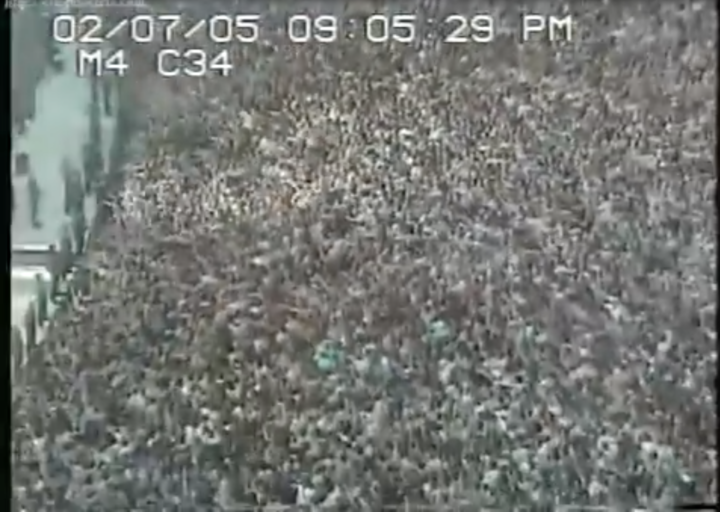
\includegraphics[width=12cm]{srowd.png}\\
    Figure 1 - Oasis concert in Manchester, England in 2005
\end{center}
If a mechanical wave propagates in a solid thin rod, the speed of sound is determined by the Newton-Leibniz equation:
\[ c = \sqrt{\frac{E}{\rho}}\]
where: c - speed of sound\\
E - Young modulus\\
$\rho$ - Material density\\\\
The average crowd density can be calculated as:
\[ \rho=\frac{m \cdot d }{h}=\frac{62kg \cdot 3.43 m \textsuperscript{-2}}{1.72 m}=123.64\frac{kg}{m \textsuperscript{3}}\]
where: m - average human mass\\
d - planar crowd density (people per square meter)\\
h - average human height\\\\
Thus, from the Newton-Leibniz equation:
\[ E = c\textsuperscript{2} \cdot \rho = 10.43\frac{m\textsuperscript{2}}{s\textsuperscript{2}} \cdot 123.64\frac{kg}{m \textsuperscript{3}} = 1290 \frac{N}{m\textsuperscript{2}}\]\\
Therefore, it is possible to compute human to human the stiffness coefficient as:
\[K = \frac{E\cdot S}{L}\]
where: S - average square of interaction between two humans\\
L - average distance between two people\\\\
At the same time, an average square of interaction between two humans can be computed as a multiplication between the average human height and the average distance between two humans. Then stiffness coefficient is equal to:
\[K = E \cdot h = 1290 \frac{N}{m\textsuperscript{2}} \cdot 1.72 m = 2219\frac{N}{m}\]
 It is possible to build a mass-spring-dumper chain (figure 2) with obtained elasticity and average human mass, to simulate generalized crowd behavior.
 \begin{center}
    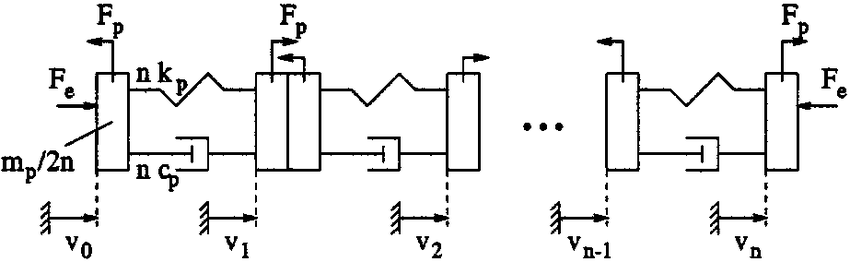
\includegraphics[width=12cm]{Model.png}\\
    Figure 2 - Mass-spring-damper chain
\end{center}
\[m \ddot x + b \dot x + Kx = 0\]
where x - vector of humans positions\\
b - damper factor\\\\
It is impossible to find the damper factor in the studied video because the crowded area was smaller than the wave-decreasing length. But it is understandable that it is small enough for our study. On the other side, the damping factor is important for system stability. It is necessary to set damping factor based on heuristic considerations such small that the general behavior was the same or changed insignificantly.\\\\
Let's check the correctness and applicability of assumptions by making a computer model based on obtained parameters and measuring wave velocity.
To do that, let's make a virtual area 10 by 3 meters (figure 3). It must contend $3.43\cdot10\cdot3=103$ people. It makes up 3.4 meters per second. It is faster by 5\% than the original one. The deviation is due to measurement error.
\begin{center}
    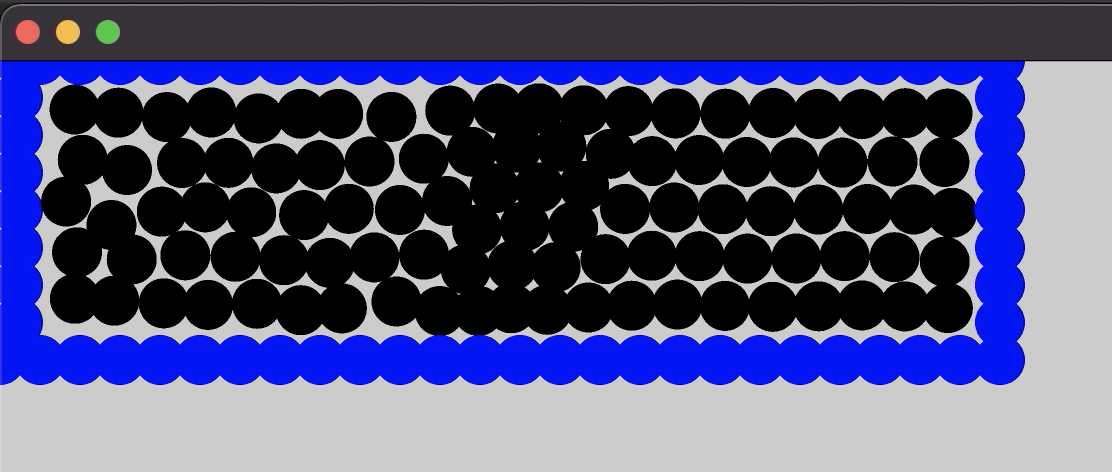
\includegraphics[width=12cm]{Wave.png}\\
    Figure 3 - Crowd model (wavefront in the middle)
\end{center}
\chapter*{Crowd control}
\section*{Crowd detection}
The first problem is detecting crowded areas. Which area is called crowded? If there is exist a situation where human is blocked from all sides, such human and all people around them formed a crowded area.\\\\
Let's make several assumptions:
\begin{enumerate}
    \item Everyone in the crowd has a smartphone
    \item Some smartphones may interconnect with each other locally
    \item Some smartphones may has a considered application
\end{enumerate}
In the trivial case, every smartphone has an application. It can communicate with other smartphones and share geolocation.













\chapter*{Bibliography}
1. Arriola-Rios, Veronica E. and Guler, Puren and Ficuciello, Fanny and Kragic, Danica and Siciliano, Bruno and Wyatt, Jeremy L., "Modeling of Deformable Objects for Robotic Manipulation: A Tutorial and Review", Frontiers in Robotics and AI 2020\\
2. Song, Y., and Bai, L. (2008). “3D modeling for deformable objects,” in Articulated Motion and Deformable Objects, Proceedings (Mallorca), Vol. 5098, 175–187. doi: 10.1007/978-3-540-70517-818\\
3. Sederberg, T. W., Zheng, J., Bakenov, A., and Nasri, A. (2003). "T-splines and t-nurccs", ACM Trans. Graph. 22, 477–484. doi: 10.1145/882262.882295\\
4. D. De Gregorio, G. Palli, and L. Di Stefano, “Let’s take a walk on superpixels graphs: Deformable linear objects segmentation and model estimation”, in Lecture Notes in Computer Science - Asian Conference on Computer Vision. Springer, 2018, pp. 662–677.\\
5. Frangi, A.F., Niessen, W.J., Vincken, K.L., Viergever, M.A.: Multiscale vessel
enhancement filtering. In: International Conference on Medical Image Computing
and Computer-Assisted Intervention, Springer (1998) 130–137\\
6. Staal, J., Abra`moff, M.D., Niemeijer, M., Viergever, M.A., Van Ginneken, B.:
Ridge-based vessel segmentation in color images of the retina. IEEE transactions
on medical imaging 23 (2004) 501–509\\
7. Gurdjos P., Von Gioi R.G.: A parameterless line segment and
elliptical arc detector with enhanced ellipse fitting. In: Computer Vision–ECCV
2012. Springer (2012) 572–585\\
8. A. Caporali, R. Zanella, D. De Gregorio and G. Palli, "Ariadne+: Deep Learning-based Augmented Framework for the Instance Segmentation of Wires," in IEEE Transactions on Industrial Informatics, doi: 10.1109/TII.2022.3154477. \\
9. A. Caporali, K. Galassi and G. Palli, "3D DLO Shape Detection and Grasp Planning from Multiple 2D Views," 2021 IEEE/ASME International Conference on Advanced Intelligent Mechatronics (AIM), 2021, pp. 424-429, doi: 10.1109/AIM46487.2021.9517655.\\
10. Jan Matas, Stephen James, Andrew J. Davison "Sim-to-Real Reinforcement Learning for Deformable Object Manipulation", Proceedings of The 2nd Conference on Robot Learning, PMLR 87:734-743, 2018.\\
11. Yilin Wu, Wilson Yan, Thanard Kurutach, Lerrel Pinto, Pieter Abbeel "Learning to Manipulate Deformable Objects without Demonstrations", University of California, Berkeley 2020\\
12. D. Seita, A. Zeng, "Learning to Manipulate Deformable Objects", Google AI blog 2021\\
13. Z. Hu, T. Han, P. Sun, J. Pan, and D. Manocha "3D Deformable Object Manipulation using Deep Neural Networks", IEEE ROBOTICS AND AUTOMATION LETTERS 2019\\
14. Frank, B., Stachniss, C., Schmedding, R., Teschner, M., and Burgard, W. (2014). Learning object deformation models for robot motion planning. Robot. Auton. Syst. 62, 1153–1174. doi: 10.1016/j.robot.2014.04.005\\
15. A. Tasora, R. Serban, A. Pazouki, D. Melanz. "Chrono: An open source multi-physics dynamics engine", 2016 Conference Paper in Lecture Notes in Computer Science. \\
16. O. Roussel, M. Taïx. “Deformable Linear Object manipulation planning with contacts.”, Robot Manipulation: What has been achieved and what remains to be done? Full day workshop at IEEE/RSJ International Conference on Intelligent Robots and Systems (IROS), Sep 2014, Chicago, United States

\end{document}
